\documentclass{article}
\usepackage{multirow}% http://ctan.org/pkg/multirow
\usepackage{hhline}% http://ctan.org/pkg/hhline
\usepackage[numbers]{natbib}
\usepackage{amsfonts}
\usepackage{graphicx}
\usepackage{tikz}
\usetikzlibrary{calc,shapes.geometric, arrows,positioning, decorations.shapes}
\tikzstyle{process} = [ellipse, rounded corners, minimum width=2cm, minimum height=1cm,text centered, draw=black, fill=white,]
\usepackage{blindtext}
\usepackage{fixltx2e}
\usepackage{caption}
\usepackage{subcaption}
\renewcommand\thesubfigure{\alph{subfigure}}
\usepackage{amssymb}
\usepackage{pdfpages}
\usepackage{hyperref}
\usepackage{amsmath}
\usepackage{graphicx}
\usepackage{epstopdf}
\usepackage{amsmath}
\usepackage{float}
\usepackage{enumitem}
\usepackage{relsize}
\usepackage{hyperref}

\hypersetup{
    colorlinks=true,
    linkcolor=black,
    citecolor=black,
    filecolor=black,
    urlcolor=black,
}
\usepackage[utf8]{inputenc}
\usepackage[english]{babel}
 
\usepackage{amsthm}
 
\theoremstyle{definition}
\newtheorem{definition}{Definition}
\newtheorem{theorem}{Theorem}[section]
\newtheorem{corollary}{Corollary}[theorem]
\newtheorem{lemma}{Lemma}
 
 
 \title { \Large{ \textbf {Performance analysis of a beauty parlour}}} 
\date{ }
\begin{document}
 \maketitle 
\begin{center}{Ankita Nanda \break Professor: Dr. Elisa Schaffer}\break
 \small \textit {Universidad Aut{\'o}noma de Nuevo Le{\'o}n}\break\break \break
 \large{ \textbf {Abstract}}
\end{center}



\section{Problem definition}
Beauty parlour is a growing business now a days in Mexico. But due to the large numbers of beauty parlour leads to a big competition in the market. In today's first moving world, people want good quality service in less time and minimum cost as well. Customer always want that expected wait is short and they join the parlour to receive the service when the queue is small. So, it is very important for a beauty parlour owner to identify a optimum matching of cost and time so as to gain high revenue while providing an efficient service to the customer. If the traffic congestion is very high to the level that customer can tolerate, then he/she should take proper action to reduce this congestion so that customer won't leave the parlour without getting service.
	In this project, our objective is to apply queuing theory techniques to the beauty parlour in order to maximize efficiency of the parlour in term of cost and waiting time of the customer. This project will support the owner of the parlour in terms of decision making for reducing the waiting time of customers to receive service, by solving a simulation model with the help of queuing theory.

\section{Objective}
The overall objective of this project is to develop a model so as caclculate the different performance measures of the system which will be used to achieve the following goals.

\begin{itemize}
\item To reduce the waiting time of the customers if it is higher than a certain value.
\item To check if persons should be hired or fired to optimize the quality-efficiency trade-off. 
\item To check if the capacity of the waiting room be increased so as to provide more space for the customer to sit.

\end{itemize} 

\section{Data}
The data used for this project belongs to a beauty parlour called Ali's beauty parlour located in San pedro, Monterrey, Nuevo Leon, Mexico. The beauty parlour is opened from Monday to Saturday between 8:00 am to 7:00 pm. Data are being collected by the beauticians of the parlour for two weeks starting from 10-01-2014 to 22-02-2014. The departure time is recorded is the time when the client finished the service. So the time taken to pay the bill for the service at the counter is not taken into account. So, when a client finishes her service, the client is assumed to depart from the system.

\section{Process details}

In the beauty parlour system, a customer comes and enters to the waiting queue. If there is no one in the queue waiting, he/she enter directly to receive the service without waiting. If there are other customer waiting in the queue or all the servers are busy, than she has to wait until her turn. Once it is her turn, she goes into one of the vacant server to receive service. After her service is finished she pays and goes out of the system. Customers are served in a first come first serve discipline (FCFS). The map of the process is given as follow.

\begin{figure}[H]
\includegraphics[trim={0cm 15cm 0cm 1cm},clip,scale=0.5]{C:/Users/Arun/Desktop/project_elisa/figures/map.pdf}{\centering}
\caption{Map of the process}
\label{fig:map}
\end{figure}



\section{Terminologies used to develop the model}
\begin{itemize}
\item Mean arrival rate= $ \lambda $ 
\item Mean service rate of a server =  $\mu$ 
number of servers = n
\item Offered load per server = $r$
\item Traffic intensity = $ \rho $
\item Empty system probability = $ p_{0} $
\item Expected number of customers in service = $ L_{s} $
\item Expected number of customers in the system = $ L $
\item Expected number of customers in queue = $ L_{q} $
\item Expected number of customers in service = $ L_{s} $
\item Mean total time in the system = $ W $
\item Mean service time = $ L_{s} $
\item Mean waiting time in the queue time = $ L_{q} $
\end{itemize}

\section{Assumptions made to develop the model}
\begin{itemize}
\item Inter-arrival times are exponentially distributed with rate $\lambda$.
\item Service times are exponentially distributed with rate $\mu$.
\item There are no waiting capacity constraints in the parlour i.e the system has infinite capacity.
\item Service skill of all the employees is assumed to be the same i. e all the servers are identical in terms of proving service.
\end{itemize}	

\section{Queueing model}
In the beauty parlour under our study as there are four persons available for receiving the clients. So, the number of servers is 4. There are seven chairs available for the customers to sit and wait if there is crowd. But there is no limit on the number of incoming customers. So, our queuing system has infinite capacity. 
	The queuing model proposed for this project is a $ M/M/3/\infty/FCFS $ model where arrival pattern is Markovian ($M$) i.e. inter arrival time is exponentially distributed with mean $\lambda $. Service time distribution is Markovian ($M$) i.e. service time is exponentially distributed with mean 
 $\mu$ . Queue discipline is First Come First Served ($FCFS$). System capacity is $ \infty $ i.e. there is no limit to the number of customers allowed to the beauty parlour. Number of parallel servers is 4 i.e. there are four persons in the parlour to attend the clients.

\section{Flow diagram}

The following diagram tells the rate with which transition between the states in the system occurs.

\begin{figure}[H]
\includegraphics[trim={2cm 19cm 0cm 4cm},clip,scale=0.7]{C:/Users/Arun/Desktop/project_elisa/flow.pdf}{\centering}
\caption{Transitions between different states}
\label{fig:flow}
\end{figure}

The circles with the text inside represents the state of the system i.e numbers of clients present in the beauty parlour. The mean arrival rate and mean departure rate of the entire system is given as:

\[
\lambda_s = \lambda \text{ where } \lambda_s \text{ arrival rate to the entire system.}
\]

 \[
    \mu_s=\left\{
                \begin{array}{ll}
                  n\mu  \text{ for } 1 \leq n < 4\\
                    \\
                  4\mu \text{ for } n\geq 4 
                \end{array}
              \right.
              \text{ where } \mu_s \text{ departure rate from the entire system.}
  \]

\section{Exploratory analysis}
First the number of counts for different days are plotted separately for two weeks. The histogram for the arrival counts of two weeks is given as follows.

\begin{figure}[H]
\hspace{1.5cm}
\noindent 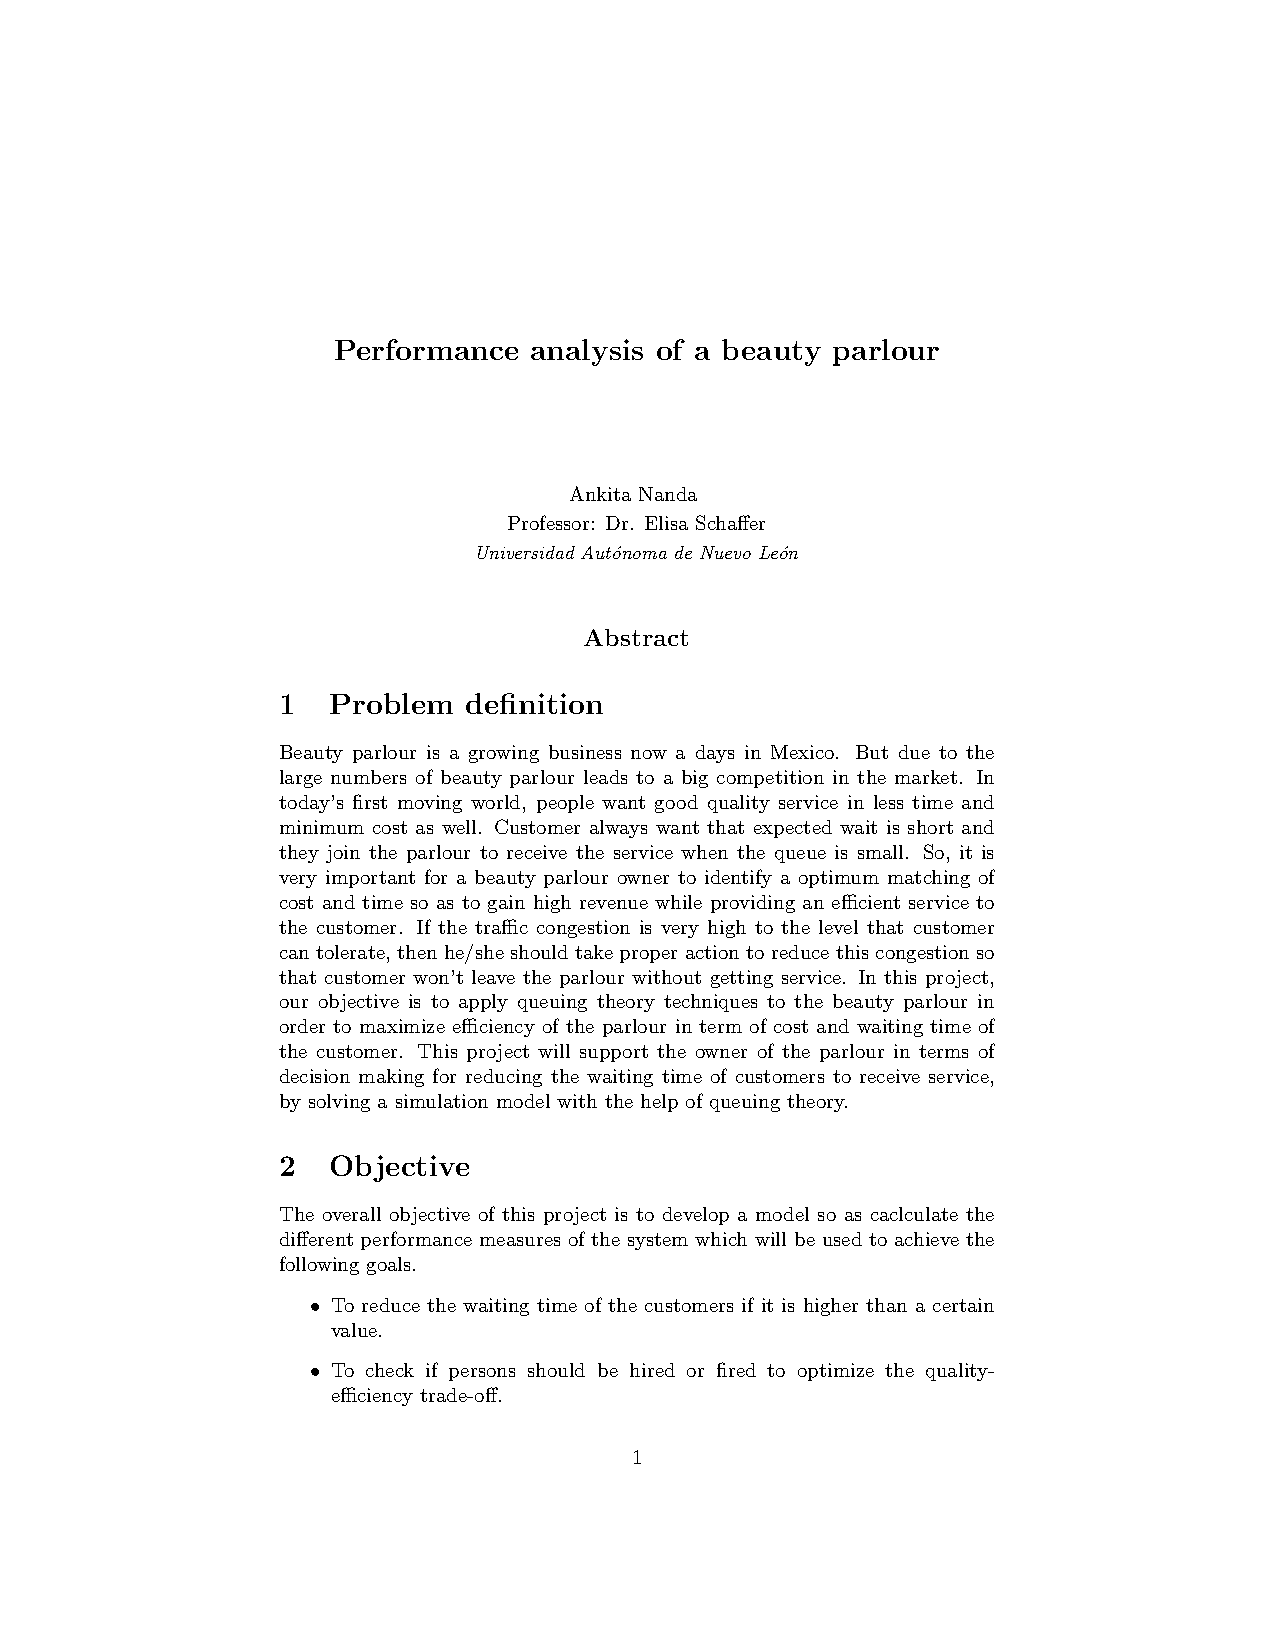
\includegraphics[scale=0.7]{C:/Users/Arun/Desktop/project_elisa/project.pdf}{\centering}
\caption{Histograms of customers arrival counts}
\label{fig:hist}
\end{figure}

From the Figure \ref{fig:hist} the graph it is clear, that more number of clients arrive to the parlour in week ends as compared to week ends. This was also confirmed for the owner of the parlour. So, rate of arrivals
are different for week days and week ends. For this reason the analysis will be done separately for week days and week ends.

\section{Statistical analysis}

Inter-arrival time is the time between two successive arrivals. The probability distribution of inter-arrival time $ T_{a} $ is given as:
\begin{equation}
f(t;\lambda)= \lambda e^{-\lambda t}\text{ where }\lambda \text{ is the inter-arrival rate. }
\end{equation}
\begin{equation}
E[T_{a}]=\dfrac{1}{\lambda}
\end{equation}

The distribution of service time is gives as:
\begin{equation}
f(t;\mu)= \mu e^{-\mu t}\text{ where }\mu \text{ is the service rate. }
\end{equation}
\begin{equation}
E[T_{s}]=\dfrac{1}{\mu}
\end{equation}

\section{Parameter estimation}
The Method of Moment \textit{(MOM)} estimation technique will be used to estimate the value of $ \lambda $ and $ \mu $.This is a statistical estimation technique that uses the moments of the sample of data to estimate the parameters. First a set of equations of the parameters will be found in terms of moments of the sample. Then those equations will be solved to get the parameters of the queuing model.As per MOM, the estimates of $ \lambda $ and $ \mu $ based on the first two moments of the data are given as below.

\begin{equation}
\lambda =\sqrt{\dfrac{1}{m_{2}-m_{1}^{2}}} \text{ where } m_{1}= E[T_{a}] \text{ and } m_{2}= E[T_{a}^{2}]
\end{equation}

\begin{equation}
\mu =\sqrt{\dfrac{1}{m_{2}-m_{1}^{2}}} \text{ where } m_{1}= E[T_{s}] \text{ and } m_{2}= E[T_{s}^{2}]
\end{equation}

\section{Measure of Performances}
\begin{equation}
r=\dfrac{\lambda}{\mu}
\end{equation}
\begin{equation}
\rho=\dfrac{r}{n}
\end{equation}
\begin{equation}
p_{0}=\bigg(\dfrac{r^{n}}{c!(1-\rho)^{2}}  + \sum_{k=0}^{k=n-1}\dfrac{r^{k}}{k!}\bigg) 
\end{equation}
\begin{equation}
L_{s}=r=\dfrac{\lambda}{\mu}
\end{equation}
\begin{equation}
L=r+ \bigg(\dfrac{r^{n}}{c!(1-\rho)^{2}}\bigg)p_{0}
\end{equation}
\begin{equation}
L_{q}=L-L_{s}
\end{equation}
\begin{equation}
W=\dfrac{L}{\lambda}
\end{equation}
\begin{equation}
W_{s}=\dfrac{L_{s}}{\lambda}
\end{equation}
\begin{equation}
W_{q}=W-W_{s}
\end{equation}


\section{Result}

The estimated parameters and measures of performances for week days and week ends are listed in the following tables.
\begin{center}
\scalebox{0.9}{
 \begin{tabular}{| c | c | c | c | c | c | c | c | c | c | c | c |} 
 \hline 
 \multicolumn{12}{|c|}{\textbf{Week days} } \\ 
 \hline
 $\lambda$ & $\mu$ & n & r & $\rho$ & $p_{0}$ & $L$ & $L_{s}$ & $L_{q}$ & $ W$ & $W_{s}$ & $W_{q}$  \\ [0.5ex] 
 \hline
 0.026 & 0.017 & 4 & 1.529 & 0.382 & 0.618 & 2.127 & 0.598 & 1.529 & 81.808 & 22.984 & 58.824 \\ [0.5ex] 
 \hline
  \multicolumn{12}{|c|}{\textbf{Week ends}} \\ 
 \hline
 $\lambda$ & $\mu$ & n & r & $\rho$ & $p_{0}$ & $L$ & $L_{s}$ & $L_{q}$ & $ W$ & $W_{s}$ & $W_{q}$  \\ [0.5ex] 
 \hline
 0.026 & 0.017 & 4 & 1.529 & 0.382 & 0.618 & 2.127 & 0.598 & 1.529 & 81.808 & 22.984 & 58.824 \\
 \hline
 
\end{tabular}}
\label{table:1}
\end{center}


From Table \ref{table:1} , it was found that on week days a customer has to wait on an average 1.67 minutes while on week ends mean waiting time in the queue is 22.98 minutes to receive service. So the system is very poor in terms of quality on week ends. The utility of the server ($\rho$) is 0.191 in week days and 0.382 in week ends respectively. So the server utility is only $19\%$ on week days and $38\%$ on week ends. From this we can say that the the system is not efficient on week days. The same conclusion can be done from the empty system probability $p_{0}$ which is found to be 0.809 on week days and 0.618 on week ends. So, on an average around $80\%$ of the time the entire system is ideal on week days This also points that the system is very bad in terms of efficiency on week days.
	The efficiency of the system can be increased by augmenting the percentage of server utility ($\rho$). To do this, first maximum waiting time of the customer in the queue $(W_{q})$ has to be fixed. For this project value of $W_{q}$ is taken to be 15 minutes. $W_{q}$ will be calculated for different number of servers decreasing the number of server one by one while keeping the value of $\rho$ less than one. This process will be continued until the calculated waiting time is less than or equal to  $W_{q}$ to get the optimum number of server. The result of this process is given in the following table.

\begin{center}
\scalebox{0.78}{
 \begin{tabular}{| c | c | c | c | c | c | c | c | c | c | c | c |} 
 \hline
 \multicolumn{12}{|c|}{\textbf{Week days}} \\
  \hline
 $\lambda$ & $\mu$ & n & r & $\rho$ & $p_{0}$ & $L$ & $L_{q}$ & $L_{s}$ & $ W$ & $W_{q}$ & $W_{s}$  \\ [0.5ex] 
 \hline
 \multirow{4}{*}{0.013} & \multirow{4}{*}{0.017}  & 4 & \multirow{4}{*}{0.765}  & 0.191  & 0.809  & 0.786  & 0.022  & \multirow{4}{*}{0.765}  & 60.499  & 1.675 & \multirow{4}{*}{58.824} \\
 \multirow{4}{*}{} & \multirow{4}{*}{} & 3 & \multirow{4}{*}{}  & 0.255  & 0.745  & 0.899  & 0.134  & \multirow{4}{*}{} & 69.15  & 10.327  & \multirow{4}{*}{}\\
 
 \multirow{4}{*}{} & \multirow{4}{*}{} & 2 & \multirow{4}{*}{} & 0.382  & 0.618  & 1.531  & 0.766  & \multirow{4}{*}{} & 117.78  & 58.957  & \multirow{4}{*}{} \\

\multirow{4}{*}{} & \multirow{4}{*}{}  & 1  & \multirow{4}{*}{}  & 0.765  & 0.235  & 14.577  & 13.812  &\multirow{4}{*}{} & 1121.324  & 1062.5  & \multirow{4}{*}{}\\
 \hline
\end{tabular}}
\label{table:2}
\end{center} \multirow{4}{*}{}

\begin{center}
\scalebox{0.78}{
 \begin{tabular}{| c | c | c | c | c | c | c | c | c | c | c | c |} 
 \hline
 \multicolumn{12}{|c|}{ \textbf{Week ends}} \\
  \hline
 $\lambda$ & $\mu$ & n & r & $\rho$ & $p_{0}$ & $L$ & $L_{q}$ & $L_{s}$ & $ W$ & $W_{q}$ & $W_{s}$  \\ [0.7ex] 
 \hline
  \multirow{4}{*}{0.026} & \multirow{4}{*}{0.017} & 4 & \multirow{4}{*}{1.529} & 0.382 & 0.618 & 2.127 & 0.598 & \multirow{4}{*}{1.529} & 81.808 & 22.984 & \multirow{4}{*}{58.824} \\
  \multirow{4}{*}{} & \multirow{4}{*}{} & 3 & \multirow{4}{*}{} & 0.51 & 0.49 & 4.011 & 2.481 & \multirow{4}{*}{} & 154.259 & 95.435 & \multirow{4}{*}{} \\
  \multirow{4}{*}{} & \multirow{4}{*}{} & 2 & \multirow{4}{*}{} & 0.765 & 0.235 & 22.654 & 21.125 & \multirow{4}{*}{} & 871.324 & 812.5 & \multirow{4}{*}{} \\
 \multirow{4}{*}{} &\multirow{4}{*}{} & 1 & \multirow{4}{*}{} & 1.529 & --- & --- & --- & \multirow{4}{*}{} & --- & --- & \multirow{4}{*}{} \\
 \multirow{4}{*}{} &\multirow{4}{*}{} & 5 & \multirow{4}{*}{} & 0.306 & 0.694 & 1.674 & 0.145 & \multirow{4}{*}{} & 64.39 & 5.567 & \multirow{4}{*}{} \\
 \hline
\end{tabular}}
\label{table:3}
\end{center}
	
	
From the tables, it can be seen that for week days the system can work even if with one server making server utility up to 76.5 percent but then the customer's waiting time will be around 18 hours which is not at all acceptable. When the number of server is 2, the system utility can be increased to around $38\%$ and the customer's waiting time is around 1 hour which is again very high. But when number of server is 10 minutes which is less then our fixed value of $W_{q}$ i.e 15 minutes. So for week days three servers are found to be ideal for the beauty parlour making the system utility around $25\%$. On the other hand for week ends we can see that at least two servers are needed to maintain the stable queuing system as one server will make the value of $\rho$ less than one making the system to explode. But when there are two servers again the customer has to wait for a long time around 13.5 hours and which is very high. Even if with four servers the expected waiting time of the customer is found to be around 22 minutes which is greater than $W_{q}$.But when the number of server is five, the expected waiting time of the customer is found to be around five minutes and server utilization will be $30\%$.  So, week ends an extra person should be hired to achieve a maximum wait of 15 minutes. 


\section{Conclusion}
Determining the optimum number of server depends on the case under study. For some cases number of server is chosen so as to fix a constant traffic intensity ($\rho$). For other cases number of server is chosen so that measure of congestion will be kept fixed. For this project the parameter that is used to calculate an optimum number of server is the average waiting time of the customer in the queue $W_{q}$. Applying this method the optimum number of server are found to be 3 and 5 for week days and week ends respectively.There are five chairs in the waiting room. As the expected queue length is 0.134 and 2.481 on week days and week ends respectively taking 3 and 5 servers, we can say that the waiting room is sufficiently equipped to provide sits for the waiting customers.




\end{document}
